\documentclass[11pt]{article}
\usepackage[margin=1in]{geometry}
\usepackage{amsmath,amssymb,amsthm}
\usepackage{tikz}
\usetikzlibrary{positioning}
\newtheorem{theorem}{Theorem}
\theoremstyle{definition}
\newtheorem*{definition*}{Definition}
\newenvironment{exambox}
  {\par\medskip\noindent\begin{center}\begin{minipage}{0.92\textwidth}%
   \hrule height 1pt \vspace{4pt}\noindent\textbf{$\bigstar$ EXAM PRIORITY.} }
  {\vspace{4pt}\hrule height 1pt \end{minipage}\end{center}\medskip}
\title{Graph Theory II: Trees and Minimum Spanning Trees}
\date{}
\author{}
\begin{document}
\maketitle

\section*{Walks and Paths}

We begin with the fundamental notions of traversal in a graph.

\begin{definition*}
A \textbf{walk} in a graph $G = (V, E)$ is a sequence of vertices
\[
  u_0,\; u_1,\; \ldots,\; u_k
\]
such that $\{u_{i-1}, u_i\} \in E$ for each $i = 1, \ldots, k$.
The \emph{length} of the walk is $k$, the number of edges traversed.
\end{definition*}

\begin{definition*}
A \textbf{path} is a walk $u_0, u_1, \ldots, u_k$ in which all vertices are distinct.
\end{definition*}

Any walk from $u_0$ to $u_k$ contains a path from $u_0$ to $u_k$: whenever a vertex
is revisited, the segment between the two occurrences forms a cycle that can be
short-circuited.  Repeating this step yields a path.

\begin{center}
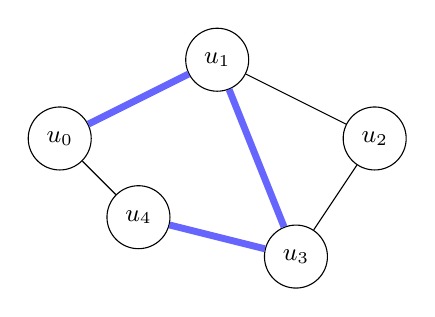
\begin{tikzpicture}[every node/.style={circle, draw, minimum size=8mm, font=\small}]
  \node (u0) at (0,0)    {$u_0$};
  \node (u1) at (2,1)    {$u_1$};
  \node (u2) at (4,0)    {$u_2$};
  \node (u3) at (3,-1.5) {$u_3$};
  \node (u4) at (1,-1)   {$u_4$};
  \draw (u0) -- (u1);
  \draw (u1) -- (u2);
  \draw (u2) -- (u3);
  \draw (u3) -- (u4);
  \draw (u4) -- (u0);
  \draw (u1) -- (u3);
  \draw[line width=2.5pt, blue!60] (u0) -- (u1) -- (u3) -- (u4);
\end{tikzpicture}

\smallskip
{\small Thick blue edges: path $u_0 \to u_1 \to u_3 \to u_4$ inside the graph.}
\end{center}

\begin{exambox}
Know the distinction between a \textbf{walk} and a \textbf{path}.
A walk may revisit vertices and edges; a path visits each vertex at most once.
Be able to identify or extract a path from a given walk.
\end{exambox}

\section*{Trees}

\begin{definition*}
A \textbf{tree} is a connected, acyclic graph.
A \textbf{forest} is an acyclic graph whose connected components are trees.
\end{definition*}

\begin{center}
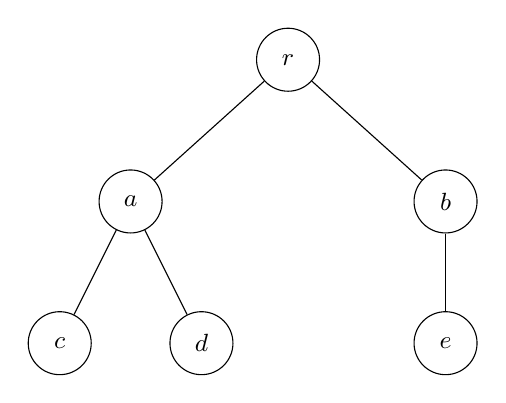
\begin{tikzpicture}[every node/.style={circle, draw, minimum size=8mm, font=\small}]
  \node (r) at (2,0)       {$r$};
  \node (a) at (0,-1.8)    {$a$};
  \node (b) at (4,-1.8)    {$b$};
  \node (c) at (-0.9,-3.6) {$c$};
  \node (d) at (0.9,-3.6)  {$d$};
  \node (e) at (4,-3.6)    {$e$};
  \draw (r) -- (a);
  \draw (r) -- (b);
  \draw (a) -- (c);
  \draw (a) -- (d);
  \draw (b) -- (e);
\end{tikzpicture}

\smallskip
{\small A tree on $6$ vertices and $5 = 6-1$ edges.}
\end{center}

\begin{theorem}
Every tree with $n \geq 1$ vertices has exactly $n - 1$ edges.
\end{theorem}

\begin{proof}
By induction on $n$.

\textbf{Base case} ($n = 1$). A single vertex has no edges, and $1 - 1 = 0$.

\textbf{Inductive step}. Assume every tree on $n$ vertices has $n - 1$ edges.
Let $T$ be a tree on $n + 1$ vertices.

Since $T$ is connected and acyclic with at least two vertices, it has at least one
\emph{leaf} (a vertex of degree~1). Let $v$ be a leaf of $T$, and let $T'$ be the
subgraph obtained by deleting $v$ and its unique incident edge. We claim $T'$ is a
tree:
\begin{itemize}
  \item \emph{Acyclic.} $T'$ is a subgraph of the acyclic graph $T$.
  \item \emph{Connected.} Any path in $T$ between two vertices of $T'$ cannot pass
    through $v$: since $v$ has degree~1, a walk entering $v$ must leave by the same
    edge, violating the path property. Hence all pairwise connections survive in $T'$.
\end{itemize}
$T'$ is a tree on $n$ vertices, so by the inductive hypothesis it has $n - 1$ edges.
Restoring $v$ adds exactly one edge, giving $T$ a total of $(n - 1) + 1 = n$ edges.
\end{proof}

\begin{exambox}
\textbf{Key fact.} A tree on $n$ vertices has exactly $n - 1$ edges.
Know this, and be prepared to prove it by induction using the leaf-deletion argument
above.
\end{exambox}

\section*{Spanning Trees}

\begin{definition*}
A \textbf{spanning tree} of a connected graph $G = (V, E)$ is a subgraph
$T = (V, F)$ with $F \subseteq E$ that is a tree (connected, acyclic, on all
$|V|$ vertices).
\end{definition*}

Every connected graph has at least one spanning tree: remove edges from cycles one at
a time until none remain.

\begin{center}
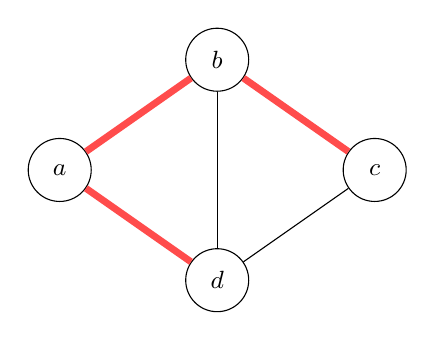
\begin{tikzpicture}[every node/.style={circle, draw, minimum size=8mm, font=\small}]
  \node (a) at (0,0)    {$a$};
  \node (b) at (2,1.4)  {$b$};
  \node (c) at (4,0)    {$c$};
  \node (d) at (2,-1.4) {$d$};
  \draw (b) -- (d);
  \draw (c) -- (d);
  \draw[line width=2.5pt, red!70] (a) -- (b);
  \draw[line width=2.5pt, red!70] (b) -- (c);
  \draw[line width=2.5pt, red!70] (a) -- (d);
\end{tikzpicture}

\smallskip
{\small All edges form $G$. Red (thick) edges form one spanning tree
($4$ vertices, $3 = 4{-}1$ edges).}
\end{center}

\section*{Minimum Spanning Trees}

\begin{definition*}
Given a connected weighted graph $G = (V, E)$ with weight function
$w : E \to \mathbb{R}$, a \textbf{minimum spanning tree} (MST) is a spanning tree
$T = (V, F)$ minimizing $w(T) = \sum_{e \in F} w(e)$.
\end{definition*}

\subsection*{Edge-Swap Lemma}

The following structural lemma underlies every efficient MST algorithm.

\begin{theorem}[Edge-Swap]
Let $T^{*} = (V, E^{*})$ be an MST of $G$, and let $e \notin E^{*}$.
Adding $e$ to $T^{*}$ creates exactly one cycle $C$.
For every $e' \in C \setminus \{e\}$,
\[
  w(e') \leq w(e).
\]
\end{theorem}

\begin{proof}
Because $T^{*}$ is a spanning tree it is connected, so adding $e = \{u, v\}$
introduces exactly one cycle: the unique $u$-$v$ path in $T^{*}$ together with $e$.

Suppose for contradiction some $e' \in C \setminus \{e\}$ satisfies $w(e') > w(e)$.
Define
\[
  T^{**} = \bigl(V,\; (E^{*} \setminus \{e'\}) \cup \{e\}\bigr).
\]
Removing $e'$ splits $T^{*}$ into two components; re-adding $e$ (which lies on the
same cycle $C$) reconnects them, so $T^{**}$ is connected. $T^{**}$ is acyclic
because $e'$ was the only edge removed from the unique cycle $C$ before $e$ was
inserted. Hence $T^{**}$ is a spanning tree, and
\[
  w(T^{**}) = w(T^{*}) - w(e') + w(e) < w(T^{*}),
\]
contradicting the minimality of $T^{*}$. Therefore $w(e') \leq w(e)$.
\end{proof}

\subsection*{Kruskal's Algorithm and the Greedy Invariant}

\begin{definition*}
\textbf{Kruskal's Algorithm.}
Initialize $S \leftarrow \emptyset$. Repeatedly select the minimum-weight edge
$e \in E \setminus S$ such that $S \cup \{e\}$ is acyclic, and set
$S \leftarrow S \cup \{e\}$. Terminate when $|S| = |V| - 1$.
\end{definition*}

\begin{theorem}[Greedy Invariant]
Let $S_m$ denote the first $m$ edges chosen by Kruskal's Algorithm.
There exists an MST $T^{*} = (V, E^{*})$ with $S_m \subseteq E^{*}$.
\end{theorem}

\begin{proof}
By induction on $m$.

\textbf{Base case} ($m = 0$). $S_0 = \emptyset \subseteq E^{*}$ for any MST~$T^{*}$.

\textbf{Inductive step.}
Assume $S_{m-1} \subseteq E^{*}$ for some MST $T^{*} = (V, E^{*})$.
Let $e$ be the $m$-th edge chosen. If $e \in E^{*}$ we are done immediately.

Suppose $e \notin E^{*}$. Adding $e = \{u, v\}$ to $T^{*}$ creates a cycle $C$.
We claim some $e' \in C \setminus \{e\}$ satisfies $e' \notin S_{m-1}$: if every
edge of $C \setminus \{e\}$ were in $S_{m-1}$, then $S_{m-1}$ would contain a
$u$-$v$ path, making $S_{m-1} \cup \{e\}$ cyclic---contradicting that the algorithm
accepted $e$. Choose such $e'$.

Since $S_{m-1} \cup \{e'\} \subseteq E^{*}$ and $E^{*}$ is acyclic, $e'$ is a valid
acyclic extension of $S_{m-1}$. The algorithm selected the minimum-weight such
extension, so $w(e) \leq w(e')$. The Edge-Swap Lemma gives $w(e') \leq w(e)$;
hence $w(e) = w(e')$. Define
\[
  T^{**} = \bigl(V,\; (E^{*} \setminus \{e'\}) \cup \{e\}\bigr).
\]
By the same connectivity and acyclicity argument, $T^{**}$ is a spanning tree with
$w(T^{**}) = w(T^{*})$, hence an MST. Since $e' \notin S_{m-1}$,
\[
  S_m = S_{m-1} \cup \{e\}
  \;\subseteq\;
  (E^{*} \setminus \{e'\}) \cup \{e\} = E^{**}.
\]
The invariant holds at step $m$.
\end{proof}

When Kruskal's Algorithm terminates it has produced a spanning tree
$T_{\mathrm{out}}$ on $|V| - 1$ edges. By the Greedy Invariant,
$T_{\mathrm{out}} \subseteq E^{*}$ for some MST $T^{*}$; since both are spanning
trees of the same size, $T_{\mathrm{out}} = T^{*}$ is itself an MST.

\begin{exambox}
\textbf{Greedy MST (Kruskal's).} At each step add the cheapest edge that does not
form a cycle; stop after $n - 1$ edges. Correctness rests on two pillars:
(1) every spanning tree on $n$ vertices has $n - 1$ edges, and (2) the Edge-Swap
Lemma---at every step the algorithm's edge set is a subset of some MST.
\end{exambox}

\end{document}